  \documentclass[10pt,twocolumn,letterpaper]{article}

\usepackage{cvpr}
\usepackage{times}
\usepackage{epsfig}
\usepackage{graphicx}
\usepackage{amsmath}
\usepackage{amssymb}
\usepackage{algorithm}
\usepackage{algpseudocode}
\usepackage[toc,page]{appendix}

% Include other packages here, before hyperref.

% If you comment hyperref and then uncomment it, you should delete
% egpaper.aux before re-running latex.  (Or just hit 'q' on the first latex
% run, let it finish, and you should be clear).
\usepackage[pagebackref=true,breaklinks=true,letterpaper=true,colorlinks,bookmarks=false,draft]{hyperref}


%%% comment \ShowNotes out to remove all colored comments defined with \newcommand below %%%
\newcommand*{\ShowNotes}{}

\ifdefined\ShowNotes
  \newcommand{\colornote}[3]{{\color{#1}\bf{#2: #3}\normalfont}}
\else
  \newcommand{\colornote}[3]{}
\fi
% maybe requires 
\usepackage[usenames]{color}
\definecolor{darkred}{rgb}{0.7,0.1,0.1}
\definecolor{darkmagenta}{rgb}{0.1,0.7,0.1}
\definecolor{cyan}{rgb}{0.7,0.0,0.7}
\definecolor{dblue}{rgb}{0.2,0.2,0.8}
\definecolor{maroon}{rgb}{0.76,.13,.28}
\definecolor{burntorange}{rgb}{0.81,.33,0}

%\newcommand {\note}[1]{\colornote{maroon}{Note}{#1}}
\newcommand {\todo}[1]{\colornote{cyan}{TODO}{#1}}
\newcommand {\lihi}[1]{\colornote{magenta}{LZ}{#1}}
\newcommand {\ayellet}[1]{\colornote{blue}{AT}{#1}}
\newcommand {\nadav}[1]{\colornote{red}{NA}{#1}}

% \cvprfinalcopy % *** Uncomment this line for the final submission

\def\cvprPaperID{****} % *** Enter the CVPR Paper ID here
\def\httilde{\mbox{\tt\raisebox{-.5ex}{\symbol{126}}}}

% Pages are numbered in submission mode, and unnumbered in camera-ready
\ifcvprfinal\pagestyle{empty}\fi
\begin{document}

%%%%%%%%% TITLE
\title{Partial Matching of 3D Shapes using Deformable Diversity}

\author{First Author\\
Institution1\\
Institution1 address\\
{\tt\small firstauthor@i1.org}
% For a paper whose authors are all at the same institution,
% omit the following lines up until the closing ``}''.
% Additional authors and addresses can be added with ``\and'',
% just like the second author.
% To save space, use either the email address or home page, not both
\and
Second Author\\
Institution2\\
First line of institution2 address\\
51
{\tt\small secondauthor@i2.org}
}

\maketitle
%\thispagestyle{empty}

%%%%%%%%% ABSTRACT
\begin{abstract}
We propose a novel approach for the matching of partial deformable shapes in 3D. Inspired by recent advances in 2D template matching techniques, our method relies on the concept of deformable diversity similarity(DDIS), extends and adapts it from an image to the 3D shape domain, and leverages the distinct behavior of this framework in different scales to achieve shape correspondences. We evaluate this framework on the SHREC16 partial matching of deformable shapes and show state of the art performance in achieving sparse correspondences.
{\color{cyan}{\bf Currently done Section 3 \& 4}}
\end{abstract}

%%%%%%%%% BODY TEXT
\section{Introduction}

%%%%%%%%%%%%%%%%%%%%%%%%%%%%%%%%%%%%%%%%%%%%%%%%%%%%%%%%%%%%%%%%%%%%%%%Problem Definition
Shape correspondence is a fundamental and challenging problem in computer vision and graphics. It has usage in various applications such as transferring texture and animation. 
Shapes rarely, if ever manifest in only one pose. While rigid transformations between surfaces is a well researched topic with many adequate solutions, a more challenging problem arises when a shape is deformed non-rigidly, a case all too common for people, animals and objects.
Moreover, the shape acquisition process almost always lead to partiality of the scanned object. Occlusions arise from different angles of acquisition, which cause an object to occlude itself, or stem from other occluding objects. 
An additional type of difficulty which might be occur is topological noise, occurring when shapes touch pn another, thus making  sensors unable to seperate them.
All of these combined give rise to the challenging problem of partial correspondences, where a deformed and incomplete shape, possibly with topological changes, has to be matched with its full version. The goal of this paper is to deal with this challenging problem.

%%%%%%%%%%%%%%%%%%%%%%%%%%%%%%%%%%%%%%%%%%%%%%%%%%%%%%%%%%%%%%%%%%%%%%%Previous Works
While in a rigid setting the problem can be solved by RANSAC and ICP like approaches\cite{rusu2009fast, holz2015registration}, extending these to non-rigid case produces mediocre results due to an underlying assumption of small deformations. 
%%%%Isometry based methods
Early methods specialized for the non-rigid problem focused on minimization of intrinsic metric distortion\cite{bronstein2006generalized,Torsello:2012:GAD:2354409.2354702} and regularity of parts\cite{Bronstein:2009:PSO:1553357.1553368,bronstein2008not}. These methods all contain with them a global assumption of isometry which holds only approximately, these tended to break down with it, and are also unable to handle extreme partiality. 
%%functional correspondences
Another family of method is based on functional correspondence. These methods model correspondences as a linear operator of a known nature between a space of functions on manifolds\cite{Ovsjanikov:2012:FMF:2185520.2185526}. These methods, originally designed for the full shape correspondence scenario have achieved state of the art results on various partial matching tasks in the recent years\cite{litany2017fully,vestner2017efficient,rodola2017partial}, and produce dense correspondence maps, but are not parallelizable, and their reliance on intrinsic metrics makes them invariant to symmetry. 

%%%%%%%%%%%%%%%%%%%%%%%%%%%%%%%%%%%%%%%%%%%%%%%%%%%%%%%%%%%%%%%%%%%%%%%Our key ideas
We take a different approach. We take advantage of the fact that while the isometric property tends to break over large distances, it usually holds approximately in limited environments. These also tend to suffer a lot less from boundary effects, especially when concentrated around the extremities of a shape. 

We can thus treat the problem of partial correspondences as matching of multiple templates, each smaller then the partial surface centered around shape landmarks. 

In addition, since point descriptors are known to be modified by partiality and deformations, instead of using them directly, we follow the approach of\cite{talmi2017template}(\textbf{DDIS}) which tackles template matching in 2D and use simple statistical assumptions on the nature of nearest neighbors between small patch descriptors, along with the assumption of an approximate conservation of distances in medium environments to obtain similarity scores between these partial shape templates.

We analyze the behavior of DDIS similarity in different scales and devise a multi scale scheme which leverages the advantages of each scale while masking their shortcomings.

%%%%%%%%%%%%%%%%%%%%%%%%%%%%%%%%%%%%%%%%%%%%%%%%%%%%%%%%%%%%%%%%%%%%%%%Our improvements
We show that using this approach, we are able to generate a set of sparse correspondences, which are less prone to symmetrical assignment than functional correspondence reliant methods, and are of superior quality on the SHREC16 Partial matching challenge\cite{cosmo2016shrec}. We then demonstrate how these sparse correspondences can be used as an input to existing functional correspondence algorithms to obtain dense correspondences or a higher quality.
%%%%%%%%%%%%%%%%%%%%%%%%%%%%%%%%%%%%%%%%%%%%%%%%%%%%%%%%%%%%%%%%%%%%%%%Our Contributions
In summary, our contributions are:
\begin{itemize}
	\item A non trivial extension of Deformable Diversity from 2 to 3 Dimensions.
	\item A modified DDIS similarity measure which is more well suited to handle matching of templates with a different number of points.
	\item An empirical analysis of DDIS behavior in different scales, leading to an improved multi-scale framework.
	\item A multi-template approach to partial matching of deformable shapes which can both produce state of the art sparse correspondences, and be used as an input to functional correspondence algorithms, significantly improving the results obtained by these.
\end{itemize}

The rest of the work is organized as follows: in section 2 we go over related works in the field of shape analysis. Section 3 introduces our Deformable Diversity framework for 3D shape matching. Experiments and results are given in section 4, and the conclusions are in section 5.

%%%%%%%%%%%%%%%%%%%%%%%%%%%%%%%%%%%%%%%%%%%%%%%%%%%%%%%%%%%%%%%%%%%%%%%
%%%%%%%%%%%%%%%%%%%%%%%%%%%%%%%% section: Related work
%%%%%%%%%%%%%%%%%%%%%%%%%%%%%%%%%%%%%%%%%%%%%%%%%%%%%%%%%%%%%%%%%%%%%%%

\section{Related work}
\label{chap:related work}


\subsection{Matching Of Deformable Surfaces}
%%[APL15] [MDK16] [SPKS16][VLR17][OBCS12][KBB13][PBB13b][KBBV15][HWG14]
%%%%%%%%%%%%%%%%%%%%%%%%%%%%%%%%%%%%%%%%%Shape Descriptors%%%%%%%%%%%%%%%%%%%%%%%%%%%%%%%%%%%%%%%%%%%%%%%%
As a fundamental problem in computer graphics and vision, an extensive body of work have been done on the matching of surfaces.
A variety of shape descriptors have been devised for this task which can be roughly divided in to 2 families. 
Extrinsic ones, such as PFH\cite{rusu2008learning}, SHOT\cite{tombari2010unique} and FPFH\cite{rusu2009fast} which are usually calculated in euclidean space and are thus sensitive to non rigid deformations, but can discern between reflections and are also more robust to noise, topological artifacts and boundary effects.
On the other hand intrinsic features such as Heat\cite{bronstein2010scale} and Wave Kernel signatures\cite{aubry2011wave} are invariant under isometric transformations, but are very sensitive to partiality and are unable to discern between symmetric parts.
These have been commonly used to generate rough correspondences between surfaces and point clouds based on their similarity, but are noisy and offer little in terms of bijectivity and continuity of the solution. a measure of global consistency using these can be achieved by solving an energy minimization of the disimilarity matrices steming from an assignment, and the auction algorithm has been commonly employed for this purpose.
%%%%%%%%%%%%%%%%%%%%%%%%%%%%%%%%%%%%%%%%%Distortion minimization%%%%%%%%%%%%%%%%%%%%%%%%%%%%%%%%%%%%%%%%%%%%%%%%
Other methods use pairwise relations between points such as geodesic distances\cite{sahilliouglu2012minimum,sahilliouglu2012scale,sahillioglu2011coarse}, and search for a configuration which minimizes the distortions of these. These methods usually carry a high complexity, both due to calculating the pairwise relations, and the combinatorial configuration search, and are thus either obtain sparse matches\cite{sahilliouglu2012minimum,sahilliouglu2012scale,sahillioglu2011coarse} to alleviate this complexity, or used strategies such as coarse to fine solutions.
%%%%%%%%%%%%%%%%%%%%%%%%%%%%%%%%%%%%%%%%%Embedding Space%%%%%%%%%%%%%%%%%%%%%%%%%%%%%%%%%%%%%%%%%%%%%%%%
Another common approach has been to embed the shapes into a different lower dimension "canonical"  space, this has been done by generalized MDS\cite{bronstein2006generalized}, an embedding into the mobius group\cite{lipman2009mobius}, or by representation in the LBO basis\cite{shtern2014matching}
 %%%%%%%%%%%%%%%%%%%%%%%%%%%%%%%%%%%%%%%%%Functional Correspondences%%%%%%%%%%%%%%%%%%%%%%%%%%%%%%%%%%%%%%%%%%%%%%%%
 A notable family of works are derived from functional correspondences. Introduced at\cite{Ovsjanikov:2012:FMF:2185520.2185526,pokrass2013sparse,kovnatsky2015functional,vestner2017efficient} these assume that functions can be mapped from one manifold to another via a linear operator, finding this transfer operator allows to embed point in a space where the ICP method can obtain correspondences. 
%%%%%%%%%%%%%%%%%%%%%%%%%%%%%%%%%%%%%%%%%Learning%%%%%%%%%%%%%%%%%%%%%%%%%%%%%%%%%%%%%%%%%%%%%%%%
Lately there has been a large body of works which employ learning methods such as Random Forests\cite{Rodola:2014:DNS:2679600.2679987} and deep learning architectures\cite{masci2016geometric,boscaini2016learning,monti2017geometric}. These show the promise of achieving state of the art performance, but require a lot of annotated data.

\subsection{Partial Matching of Deformable shapes}
The introduction of partiality adds complications which are not present in the full correspondence scenario. Spectral quantities change drastically, while geodesic paths disappear.
%%%%%%%%%%%%%%%%%%%%%%%%%%%%%%%%%%%%%%%%%Rigid partial matching%%%%%%%%%%%%%%%%%%%%%%%%%%%%%%%%%%%%%%%%%%%%%%%%
For the rigid setup, the Iterative Closest Point(ICP)\cite{Aiger:2008:CSR:1360612.1360684} algorithm, preceded by initial alignment\cite{rusu2008towards} tackle partial matching successfully. Adapting this to the rigid setup however has proved to have limited success due to the alignment which is necessary, and thus is only fit for very small non-rigid deformation.

Early works which were designed with partial matching in mind\cite{bronstein2008not,bronstein2009partial} formulated an energy minimization problem over metric distortion and regularity of corresponding parts. Following works relaxed the regularity requirement by allowing for sparse correspondences\cite{Torsello:2012:GAD:2354409.2354702,rodola2013elastic}. 
Other works\cite{sahilliouglu2012scale,sahilliouglu2012minimum} minimized the distortion metric over the shape extremities by doing combinatorial search of least distortion matches and then densify them while employing a refining scheme in the process. 

In\cite{pokrass2013partial} a bag of words point-wise descriptors on a part in conjunction with a constraint on area similarity and the regularity of the boundary length to produce correspondence less matching parts without point to point correspondences by energy minimization.

Another line of works employ machine learning techniques to learn correspondences between manifolds. 
Recently \cite{rodola2017partial} had proven that partiality induces a slanted diagonal structure in the correspondence matrix and found the Laplacian eigenfunctions from each basis which induces this structure. Current state of the art\cite{litany2017fully} uses this notion in conjunction with joint diagnolization. The main drawback of this method, shared with other intrinsic methods, is its invariance to symmetries. 

\textbf{3D Shape Descriptors} 

%%%%%%%%%%%%%%%%%%%%%%%%%%%%%%%%%%%%%%%%%%%%%%%%%%%%%%%%%%%%%%%%%%%%%%%
%%%%%%%%%%%%%%%%%%%%%%%%%%%%%%%% section: 2D Shape Matching
%%%%%%%%%%%%%%%%%%%%%%%%%%%%%%%%%%%%%%%%%%%%%%%%%%%%%%%%%%%%%%%%%%%%%%%

\subsection{Template matching in 2D}
Template matching in 2D is a well researched topic. Similarly to 3D objects are going complex deformations of pose, and are only seen partially depending on the camera point of view. Recently a series of works which use a very simplistic framework based on the statistical properties of nearest neighbors in low level feature space had made good strides in tackling this complex task.

\textbf{Best Buddies Similarity}
Great strides had been achieved in the field of 2D template matching. Best Buddies Similarity\cite{dekel2015best} is a simple framework which employs a statistical assumption - if two regions $\mathcal{N}$,$\mathcal{M}$ contain the same template patches should maintain Bi Directional Similarity. 
That is - given a point $n_i\in\mathcal{N}$ and a corresponding point $m_i\in\mathcal{M}$ they should point too each other as nearest neighbors - that is if $NN_{\mathcal{M}}(n_i)=m_j$ then on a matching template we should expect $NN_{\mathcal{N}}(m_j)=n_i$. Solving for a matching template then amounts to finding the region which has the highest count of best buddies. This amazingly simple scheme has been show to be able to handle occlusions, missing parts and complex deformations of templates.

\textbf{Deformable Diversity Similarity}
Building upon the above work, \cite{talmi2017template}  relaxed the requirement for a best buddy relation, and added a requirement for spatial coherency.

The rather cumbersome best buddy relation has been relaxed to requiring only that the diversity of the set of nearest neighbors sets between corresponding templates should be high. This is actually prerequisite to a high best buddies similarity score and serves as a rough approximation of it. For this end diversity is formally defined as:
\begin{equation}
\underset{\mathcal{N}\rightarrow\mathcal{M}}{DIS}=c\cdot |\{n_i\in\mathcal{N}:\exists m_j\in\mathcal{M},NN(m_j,\mathcal{N})=n_i\}|
\end{equation}
where $|{.}|$ denotes group size and $c=1/min(|\mathcal{M}|,|\mathcal{N}|)$ is a normalization factor. Between non corresponding windows, indeed one should expect most points to have no real corresponding point, and thus be mapped to a very and remote nearest neighbors.  On the other hand, regions containing matching objects are drawn from the same distribution, thus the diversity of nearest neighbors should be high.
To accommodate this assumption not only did they rewarded high diversity of nearest neighbors, but also penalized mapping to the same patch. To this end, another, a negative diversity measure had been defined:
\begin{equation}
\kappa_{\mathcal{M}}(n_i)=|\{m\in\mathcal{M}:NN^a(m,\mathcal{N})=n_i\}|
\end{equation}
With $x_i^a$ denoting the appearance descriptor of point $x_i$.
Thus the contribution of a patch $m_j:NN^a(m_j,\mathcal{N})=n_i$ is $exp(1-\kappa_{\mathcal{M}}(n_i))$. 
An additional observation made has been that while non isometric deformations do occur, they should be restricted, small, in real objects. With  distance on the window pixel grid between 2 nearest neighbor points defined as $r_j=d(m_j^l,n_i^l)$ with $x_i^l$ denoting the location of $x_i$ on a grid, the final Deformable Diversity Similarity formulation becomes:
\begin{equation}
\underset{\mathcal{N}\rightarrow\mathcal{M}}{DDIS}=c\sum_{m_j\in\mathcal{M}} \frac{1}{1+r_j} \cdot exp(1-\kappa (NN^a(m_j,\mathcal{N})))
\end{equation}

%%%%%%%%%%%%%%%%%%%%%%%%%%%%%%%%%%%%%%%%%%%%%%%%%%%%%%%%%%%%%%%%%%%%%%%
%%%%%%%%%%%%%%%%%%%%%%%% section: 3D Deformable Diversity Similarity
%%%%%%%%%%%%%%%%%%%%%%%%%%%%%%%%%%%%%%%%%%%%%%%%%%%%%%%%%%%%%%%%%%%%%%%
\section{General Approach}
\label{sec:approach}
\begin{figure*}[htb]
	\centering
	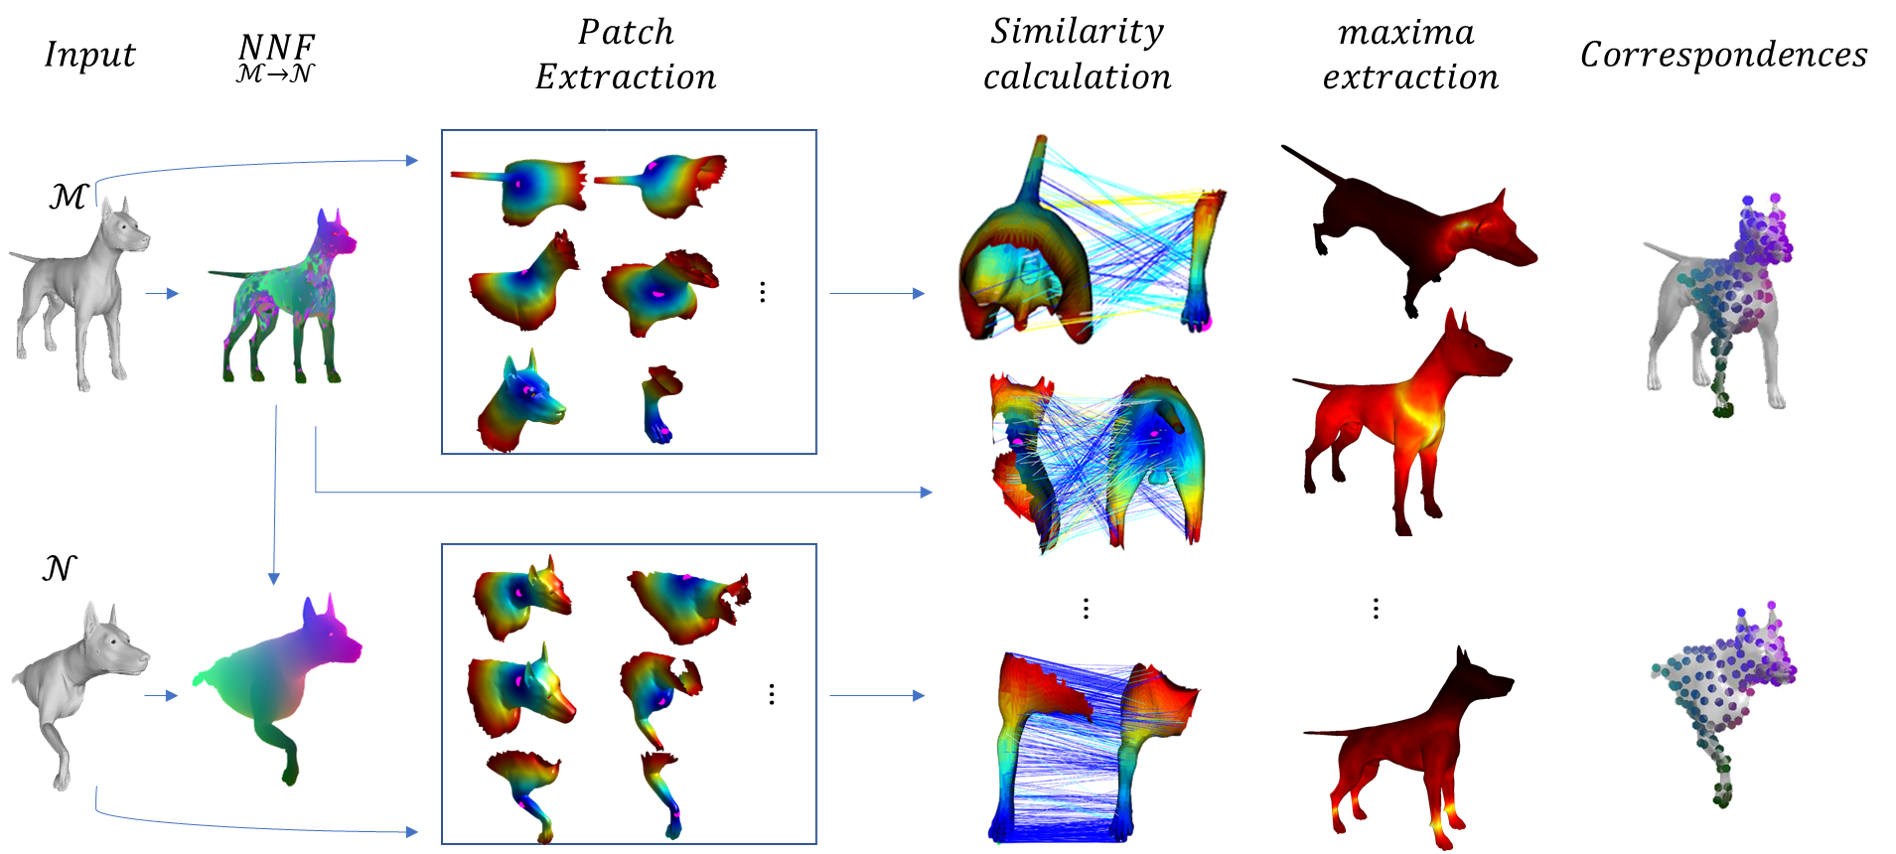
\includegraphics[width=1\textwidth]{figures/Birds_Flight.png}
	\caption{{\bf Algorithm outline.}
    In the first step, we compute the nearest-neighbor field for $\mathcal{N}$ and $\mathcal{N}$.
    Then, patches of the surfaces are extracted for every sample point in $\mathcal{N}$ and for every vertex on $\mathcal{M}$.
    These patches cover the surface (i.e., may overlap) and represent semantic regions. 
    Note that exact segmentation is not needed.
    Step 3 is the core of the algorithm, in which the similarity between the patches is computed.
    Finally, in Step 4, for every sample of $\mathcal{N}$ we set the vertex of $\mathcal{M}$ that achieves the maximal score as its corresponding point.
	\ayellet{This figure should be re-done} 
	}
	\label{fig:overview}
\end{figure*}

Given two surfaces $\mathcal{M}$ and $\mathcal{N}$, the goal is to find the best match of  $\mathcal{N}$ within  $\mathcal{M}$.
In particular, we aim at extracting a sparse set of point correspondences between the models. 
Our approach is based on three key ideas, which we describe hereafter.

%%%%%%%%%%%%%%%%%%%%Key Idea underlying the original DDIS : diversity
First, inspired by \cite{talmi2017template}, similarity is captured by two properties of the Nearest Neighbor field. 
(1) When $\mathcal{N}$ and a patch of $\mathcal{M}$ match, most points in $\mathcal{M}$ have a unique NN-match in $\mathcal{N}$. 
This implies that the NN field should be highly diverse, in the sense that many different points in $\mathcal{N}$are being matched.
(2) Arbitrary matches typically imply a large deformation, whereas correct matches should preserve the distance between pair of points.
Therefore, Similarity should be based both on the diversity of the Nearest-Neighbor field and on the consistency of the distances between the points.

% One key to our method is the assumption that while non rigid deformations and partiality leads to changes in the data, the underlying shape distributions from which the shapes on the surfaces are drawn should remain highly overlapping, and thus the data points drawn from these should be spread approximately uniformly, one inside the other, leading to a high diversity of nearest neighbors.
% %%%%%%%%%%%%%%%%%%%%%The idea underlying our improvement%%%%%%%%%%%%%%%%%%%%%%%%%%%%
% However, since unlike in\cite{talmi2017template} we don't have the benefit of having a template and a query of the same size in the absence of a grid, and the space of geometric shapes is more constrained then that of RGBXY, one should not expect a near bijection. 
%%%%%%%%%%%%%%%%%%%%Key Idea underlying the original DDIS : low deformation%%%%%%%%%
% Another assumption is that of a geometrical coherency  - geodesic distances of corresponding pairs of points on a shape and a roughly isometrically deformed version of which should hold approximately leading us to use the assumption of low distortion.
%%%%%%%%%%%%%%%%%%%%%%%%%%%%%Our added observation%%%%%%%%%%%%%%%%%%%%%%%%%%%%%%%%%
% However, the preservation of distances holds only approximately even for full template matching, and even less so in the presence of partiality and topological noise.
% It holds that the longer a distance between 2 points is, the more likely it is that a distortion had occurred on the geodesic path between them, either due to a non isometric deformation, partiality removing a piece of the geodesic path or topological noise introducing a shortcut.
% It follows from this that the smaller the pieces we are trying to match will be, the higher the likelihood of pairwise distances to be preserved should be.
Second, rather the realizing the similarity test, described above, on $\mathcal{N}$ as a whole, it is preferable to perform it on a set of small sub-surfaces of $\mathcal{N}$.
This is so not only since a small sub-surfaces is more likely to exhibit consistent distances, but also since it is less likely to be matched to a repeating pattern, which would lead to smaller diversity.

Third, a multi-scale approach with respect to the size of matched sub-surfaces is beneficial.
This is so since larger surfaces contain more global context, resulting in matches which lie in a correct region, but provide poor localization. 
On the other hand, matching smaller surfaces lead to results which are better locally, but may be globally inconsistent. \ayellet {what do you mean by globally inconsistent?}

Therefore, our algorithm, which is illustrated in Figure~\ref{fig:overview}, consists of the following steps.
\begin{enumerate}
    %%%%%%%%%%%%% Step 1
    \item 
    \textbf{Pre-processing}.
    Shape descriptors are calculated for every vertex of both meshes and an approximate nearest neighbor field is computed for the vertices, as described hereafter.
    
    Many descriptors have been proposed in the literature~\cite{rusu2008towards,tombari2010unique,Sun:2009:CPI:1735603.1735621}.
    We use the FPFH~\cite{rusu2009fast}, which is robust to small deformations and partiality of the data, yet sensitive to symmetrical flips.
    \ayellet{what makes it sensitive to symmetrical flips?}
    Therefore, it addresses a major drawback of matching a right arm, for example, to the left one.
    %
    We then compute a nearest neighbor field mapping, by assigning each vertex of $\mathcal{M}$ its nearest neighbor in $\mathcal{N}$, FPFH-wise.

    %%%%%%%%%%%%% Step 2
    \item
    {\bf Patch extraction.} 
    Inline with the second key idea, we aim at extracting a meaningful set of sub-surfaces, which cover (rather than partition) the surface.
    This is done in two steps:
    First, we extract a meaningful set of points, whose neighborhoods provide a good cover of the surface. 
    We then extract the patches using this sample.
    We elaborate hereafter.
    
    To extract the sample point set, we start from the extremities of the surface, which are considered salient points.
    A vertex is considered to be an extremity if it  resides on a tip of the surface (e.g.,  tips of limbs)~\cite{katz2005mesh},
    In practice, we define them to be vertices that are local maxima of the sum of the geodesic distance functional.
    Formally, $\forall v \in S$,  let $N_v$ be the set of neighboring vertices of vertex $v$. 
    Let $GeoDist(v_i, v_j)$ be the geodesic distance between vertices $v_i$ and $v_j$ of mesh S. Vertex $v$ is an extremity if it satisfies
     \begin{equation}
        \sum_{v_i\in S} GeoDist(v,v_i)>\sum_{v_n\in S} GeoDist(v_n, v_i).
        \label{eq:extremities}
    \end{equation}

    Then, we iteratively add more samples, choosing the next sample point as follows.
    We construct a "forbidden" region around every point in the set.
    This region is a geodesic disc of radius $ 0.05\sqrt{Area(\mathcal{M})}$.
    The next point to be added to the set is a vertex whose geodesic distance to any sample point in the set is minimal and does not fall in any of the forbidden regions.
    This process stops when the entire surface is marked forbidden. 
    % The resulting set of samples is denoted as  $\S_{\mathcal{N}}\in\mathcal{N}$.

    Once the set of representing sample set is defined, a disc (sub-surface) of geodesic distance $R_T$ is extracted around each sample point, which is the sought-after set of patches.
    Specifically, $R_T=\beta\cdot \sqrt{Area(\mathcal{M})}$.
    As our approach is multiscale, $\beta$, which was found empirically by minimizing the error of correspondences on a training set, varies. 
    In practice we use $\beta=\{0.6,0.4,0.2\}$.
 
 %   \nadav{We repeat this process for every $m\in\mathcal{M}$ to create a set of geodesic discs $\{{\mathcal{M}_{m_j}^{R_T}}\}_{j=1}^{|\mathcal{M}|}$}
    
    %%%%%%%%%%%%% Step 3
    \item
    {\bf Computing similarities between pairs of patches.} 
    This step is the core of our algorithm, which realizes the first key idea.
 
    For each pair of patches of the same scale, $Q_i \subset \mathcal{M}$ and $P_i \subset \mathcal{N}$, we compute a similarity value.
    %
    Recall that our goal is to reward a nearest-neighbor field with high diversity and low deformation. 
    We will define the similarity function $DDIS$ that achieves it  in Section~\ref{sec:similarity}.
    This is done in a multi-scale manner.

    % \textbf{Refinement.} The goal of this stage is to achieve better correspondences based on simple global tests and constraints
    % \begin{itemize}
    % \item Correspondences which exhibit high distortion are determined are marked as not trusted.
    % \item For Correspondences which are deemed not trusted we search among the local maximas of the DDIS score a point which minimizes their distortion w.r.t to trusted point.
    % \end{itemize}
    
     %%%%%%%%%%%%% Step 4
   \item{\bf Extracting a sparse set of corresponding points.}
    Given the similarity values between the patches, our goal now is to extract a set of corresponding points between  $\mathcal{N}$ to $\mathcal{M}$.
    If we had a single scale, then for each sample point (the center of a patch) of $\mathcal{N}$, we would choose the vertex of $\mathcal{M}$ that maximizes the similarity function.

    In our multi-scale approach, we proceed from coarse to fine.
    Suppose that $P_i \subset \mathcal{N}$ and $Q_j\subset \mathcal{M}$ were found to have the highest similarity in a coarsest scale (i.e. $Q_j$ is the largest).
    The coarsest match is then set between $v_i \in P_i$ and $w_j \in Q_j$, where $v_i, w_j$ are the {\em geodesic centers} of  $P_i, Q_j$, respectively (i.e. the sample points that define the patches in Step 2).
    When moving to the finer scale, we replace  $Q_j$ with a smaller (finer) patch in which $w_j$ is the center and set the new $w_j$ to be the vertex on this patch that  maximizes the similarity function $DDIS$ on this patch.
    The finest $w_j$ is the corresponding point of $v_i$; see Figure~\ref{fig:multiscale}.
    
    \begin{figure}[htb]
	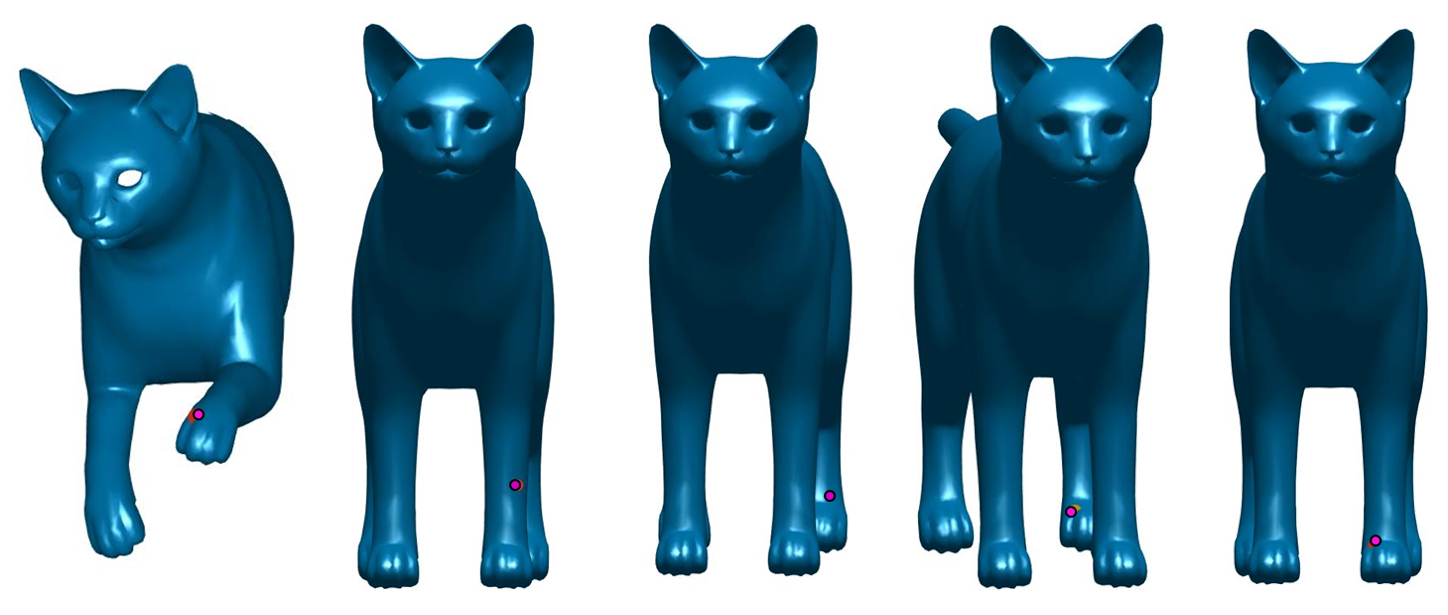
\includegraphics[width=0.5\textwidth]{figures/MultiScaleDis.png}
	\caption{{\bf Multi-scale similarity.} 
	Given the sample point on the left (in magenta), the corresponding points on  $\mathcal{M}$ are shown on the right. 
	In the coarsest level, the general region of the matching point is found, but the point is imprecise.
	In subsequent levels, the general region is not found.
	Our multi-scale approach manages to find the precise point.
	\ayellet{Replace the image.} \nadav{done}
	}
	\label{fig:multiscale}

    \end{figure}

    \item{\bf Coherency-based correspondence refinement}
    The result of Step 4 is a set of corresponding pairs of points.
    In most cases ($>92\%$ on all our examples), the correspondences are correct.
    The goal of this step is to identify the incorrect ones and replace them by the correct correspondences. 
    
    The key idea is to utilize coherency, i.e., if all points in the neighborhood of point $v \in \mathcal{N}$ are mapped to points that reside on the same region on $\mathcal{M}$,  it is expected that the corresponding point of $v$,  $w \in \mathcal{M}$, will also reside in this region.
    In other words, we are looking for outliers of the mapping.
    
    To detect these outliers, we check the sum of geodesic distances. 
    For a pair of points $(v,w)$ to be considered correct, they should satisfy:
    \begin{equation}
    \label{eq:refinement}
        \sum_{v_i\in \mathcal{M}}|{GeoDist(v,v_i)} - {GeoDist(w,w_i)}| < C
    \end{equation}
    where $w_i$ is the corresponding point of $v_i$ and $C$ is $0.15$ of the mean of Equation~\eqref{eq:refinement} on all points.
    We replace the corresponding point of an outlier by a point that minimizes Equation~\eqref{eq:refinement} and is a local maximum of the similarity function of Step 3.

\end{enumerate}

% \nadav{proposed end of section}
% \nadav{comment: This should not be in the final version .
% I had embedded this into the Similarity calculation and sparse correspondences section. hopefully it makes more sense there}
% The latter \ayellet{two steps} are performed in a multi-scale approach. 
% To do it, we define a set of $N$ scales, which define geodesic radii $R_{T_1}>...>R_{T_N}$, \ayellet{which are the pre-defined thresholds of Step 2}\nadav{No, they are not. The density of sampling radius used for step 2 is not the same as the radius we use to construct our geodesic discs}.
% The larger the radius, \ayellet{the ....}
% \ayellet{ I do not understand anything you say below. Do you use the results in one scale to calculate the other. How is Step 3 influenced?}\nadav{At step 3 we calculate k similarity scores for each pair of points - one for each geodesic disc radius $R_{T_k}$}
% \nadav{We then move from a coarse to fine scale by iteratively finding the maxima of similarity at scale $R_{T_k}$, and use to define a valid set of points from which we pick the maxima at scale $R_{T{k+1}}$ by constraining them to lie in a geodesic disc of radius $R_{T_k}$ around it. We repeat this process and determine the final correspondence at scale $N$}

%%%%%%%%%%%%%%%%%%%%%%%%%%%%%%%%%%%%%%%%%%%%%%%%%%%%%%%%%
%%%%%%%%% section: Similarity
%%%%%%%%%%%%%%%%%%%%%%%%%%%%%%%%%%%%%%%%%%%%%%%%%%%%%%%%%
\section{Similarity}
\label{sec:similarity}
\begin{figure}[htb]
	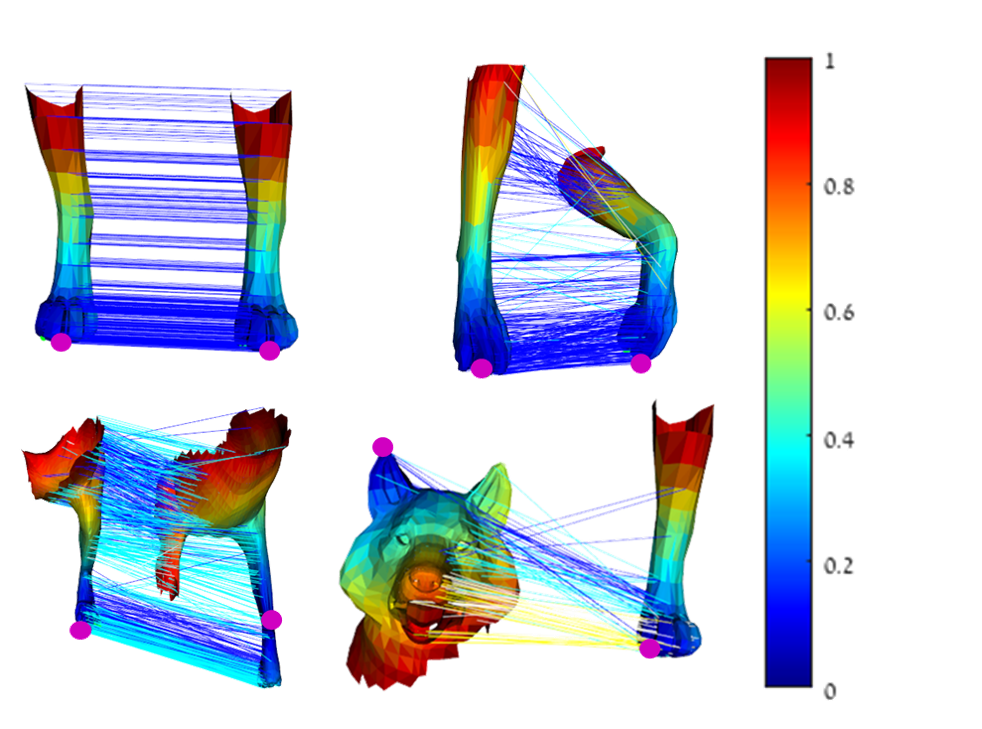
\includegraphics[width=0.5\textwidth]{figures/DDIS2.png}
	\caption{{\bf Nearest Neighbor Field.} 
		The surfaces are colored by the geodesic distances from the magenta point; the lines are colored by the \nadav{difference of geodesic distances from the purple point}. \ayellet{deviation of what?} 
		Clearly, similar surfaces on the top (even when deformed) exhibit diversity in matching (i.e. different points on one surface are matched to different points on the other).
		Furthermore, in this case, most lines are blue, which indicates similar distances from the source point.
		This is not the case at he bottom, where the surfaces are highly different from one another.
		}
		\label{fig:NNF}
\end{figure}

%Problem definition
This section elaborates on Step 3, which is the core of the algorithm.
Given pair of patches of the same scale, $Q \subset \mathcal{M}$ and $P \subset \mathcal{N}$, this section defines a similarity function, termed {\em 3D Deformable Diversity Similarity (3D-DDIS)}, between them.
This function should be oblivious to non-rigid transformation, different resolutions of the meshes, noise, and partiality of the data.

%Key idea
Recall that the key idea is to reward a point (center of the patch) whose nearest-neighbor field satisfied two properties: it has both high diversity and low deformation. 
As for diversity, when $Q$ and $P$ correspond, most of the points on $Q$ points have a unique NN-match on $P$. 
Conversely, if $Q$ and $P$ do not correspond, most of the points on $Q$  do not have a good match on $P$, and therefore the nearest neighbors are likely to belong to a small set of points that happen to be somewhat similar to the points of $Q$.
This implies that the NN-field is highly \textit{diverse}, pointing to many different points in $P$.
In addition, if two patches correspond, pairs matching (nearest neighbors) points tend to have similar geodesic distances to the centers of the patches they reside on.
Conversely, arbitrary matches typically do not maintain such distances.
\ayellet{why is it called deformation?}

To realize these requirements, we start by formally defining the diversity, $Div(Q,P)$, and  the deformation, $Def(Q,P)$, and then show how to put them together into a similarity function.
An intuitive and efficient way to measure diversity is to count the number of unique NNs between the points of  $Q$ and $P$:
\begin{equation}
\label{eq:diversity}
Div(Q,P)=|\{p_i\in P:\exists q_j\in Q,NN(q_j,P)=p_i\}|,
\end{equation}
where  $\{p_i\}_{i=1}^{|P|}$ and $\{q_j\}_{j=1}^{|Q|}$ are the set of points of $Q$ and $P$, respectively and the nearest neighbors is computed between the descriptors (FPFH) of the points.
However, we will see below that the diversity can be calculated implicitly.

Next, we define $Def(Q,P)$, the deformation from  $Q$ to $P$.
Let $p \in P$ and $q \in Q$ be the centers of $P$ and $Q$, respectively;
furthermore, let $p_i= NN(q_j,P)$ be the nearest-neighbor of  $q_j \in Q$.
The deformation implied by the NN-Field for ${p_i,q_j}$ is defined by:
\begin{equation}
def(q_j,p_i,Q,P)= |{GeodDist(q_j,q)-GeodDist(p_i,p)}\epsilon|,
\end{equation}
where $0<\epsilon << Area(\mathcal{M})$ and is a used for numerical stability.

For each $p_i \in P$, we find the minimal deformation $r_i^*=min_{q_j \in Q}def(q_j,p_i,Q,P)$ such that $p_i$ is the nearest neighbor of $q_j$.
Note that some points in $P$ might not be associated with any point in $Q$ (since they are not the nearest neighbors of any point $q_j\in Q$);
in this case $r_i^*=\infty$.

Having defined diversity between patches and deformation between points on these patches, we define the similarity between patches $p$ and $Q$ as:
\begin{equation}
DDIS(P,Q)=\sum_{p_i\in \mathcal{P}}\frac{1}{1+r_i^*}.
\label{eq:DDIS}
\end{equation}

It is easy to see how the 3D-DDIS rewards low deformation.
However, we will explain hereafter why it also rewards high diversity.
Consider a case where $r_i^*\in\{0,\infty\} \forall p_i$. 
When this occurs $\frac{1}{(1+r_i^*)}\in\{1,0\}$ and it indicates that a point $p_i$ has a point in $Q$ that considers $p_i$ to be its nearest neighbor.
In this scenario, 3D-DDIS simply counts the number of points in $Q$ that are nearest neighbors of some point in $P$.
But, this is precisely the diversity function we seek-after.
\ayellet{copy a convincing explanation for the general case}
\nadav{
In the general case, the contribution of every point is inversely weighted by its deformation $r_i^*$, which gives preference to plausible deformations of real objects.
}

%% In the thesis, in the results section add a paragraph where you explain this image
% \begin{figure}[htb]
% 	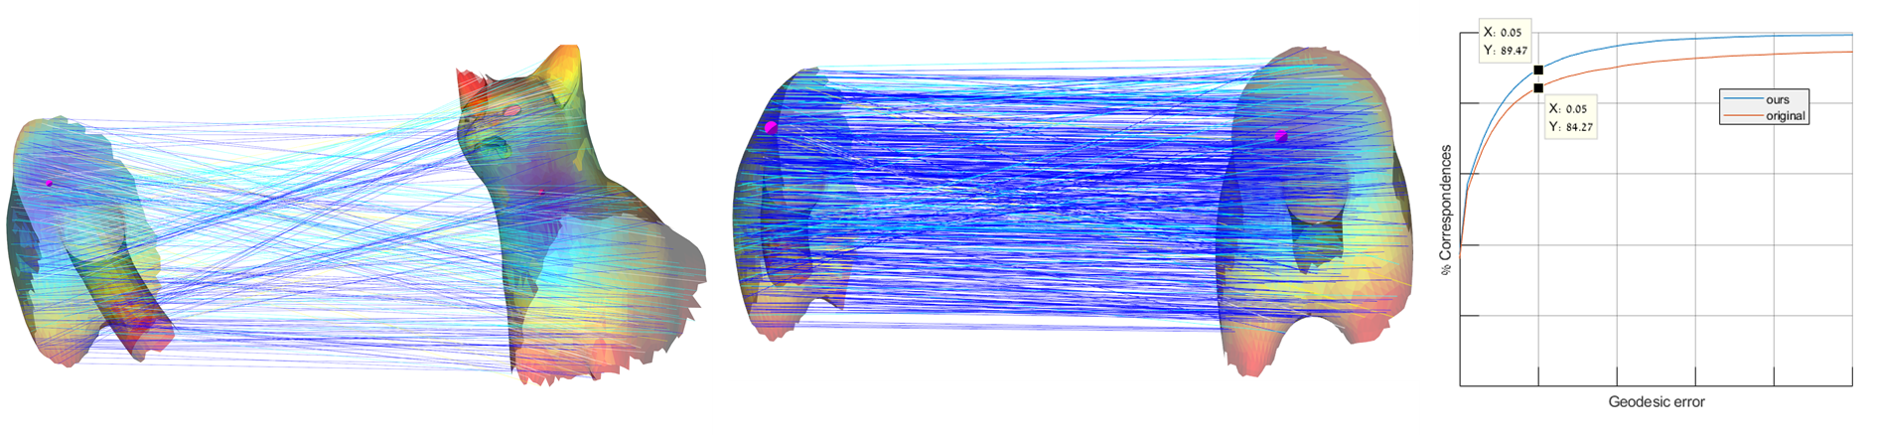
\includegraphics[width=0.5\textwidth]{figures/DDISvsWDIS.png}
% 	\caption{Qualitative and quantitative illustration of the improvement introduces by our formulation. On the top left the Nearest neighbor mapping between the part and its corresponding ground truth geodesic disc. As can be seen low distortion is occurring between the true corresponding points, but the symmetrical part which is not included on the partial model maps to the same points - thus attenuating the score originating from these. One the bottom left we see the piece chosen by the original DDIS formulation. The arrows with low distortion seldom have other points which are their nearest neighbors and thus achieves a better score without our modification. The cumulative error curves show an improvement of ~5 percent on the training set using our formulation.}
% \end{figure}

%%%%%%%%%%%%%%%%%%%%%%%%%%%%%%%
%%%%%%% Section: Results
%%%%%%%%%%%%%%%%%%%%%%%%%%%%%%%
\section{Results}
\label{section:results}

We have evaluated our method both qualitatively and quantitatively on several datasets:
(1) the benchmark of {\em SHREC'16A---partial matching of deformable shapes}~\cite{cosmo2016shrec};
(2) the even more challenging benchmark of {\em SHREC’16B---matching of deformable shapes with topological noise}~\cite{lahner2016shrec}.
\ayellet{(3) Faust, (4) Archaeology}
\nadav{(3) {\em FAUST}\cite{bogo2014faust} includes real scans of human subjects. For this set we provide only qualitative evaluation.}
\nadav{(4) {\em Archaeology} includes various scans of archaeological artifacts with repeating patters.}
In all cases, our method either outperformed the state-of-the-art methods or was competitive.

{\em SHREC'16A} contains $400$ partial shapes, each is a near-isometrically deformed version of one of eight base model, given in a neutral pose.
% Each class is provided with a "null" shape in a neutral pose. 
The dataset is further divided into two subsets, according to the type of partiality:
(1) \textit{cuts}, which is composed of shapes produced by dividing shapes by a plane, and (2) \textit{holes}, obtained by eroding many areas around random vertices. 
% The size of the parts ranges from ~800-9k vertices.
%%%%
{\em SHREC’16B} is contains $10$ shapes, which are
% with ~10K vertices each, 
derived from the same base human shape that undergoes deformations and topological changes stemming from self-intersections. 
% Each shape is matched to all the others resulting in 90 matching problems.

\nadav{{\em FAUST} contains $200$ real world scans of 10 different human subjects. The acquisition process of which introduces topological artifacts and missing parts due to occlusions.}

\ayellet{paragraph: explain that there are two distinct, yer related challenges: sparse and dense}
\nadav{Surface correspondence algorithms can divided into 2 by the density of their correspondences. 
	(1) Sparse correspondences which aim to cover the surface area uniformly, but sparsely.
	(2) Dense correspondences which match every vertex on one shape to the other shape.}
\ayellet{paragraph: explain that you compute only sparse and then use... to convert it into dense.}
 \nadav{ Our method produces sparse correspondences, yet these can be converted to dense ones with a minimal loss of quality.
 This is achieved by using the sparse correspondences as input to the method of \cite{litany2017fully}.}
\paragraph{Qualitative results:} 
Figure~\ref{fig:Shrec16Qualitative} illustrates our results on two models from {\em SHREC'16A}.
In this figure, the input model $\mathcal{M}$ is color-coded according to its coordinates.
The matches on the partial model $\mathcal{N}$ (partial models and holes) are colored according to the match.
Therefore, it is easy to visually verify if the match is correct or not.

It can be seen that our method obtains sparse correspondences of a high quality, since the dots on the model suit in color to the matching parts of $\mathcal{M}$ .
Furthermore, when comparing our dense-correspondence results to those of~\cite{rodola2017partial} (which computes dense correspondence directly), our method produces better results.
It should be noted that symmetries are less of a problem in our method, due to distance preservation between points in Equation~\eqref{eq:DDIS} (note the legs).
This is especially important when the model contains holes.
\begin{figure*}[htb]

	\centering
		\setlength\tabcolsep{0.5pt}
	\begin{tabular}[width=0.8\textwidth]{c|ccc|ccc}
	     input & sparse & dense &  \cite{rodola2017partial}
	           & sparse & dense & \cite{rodola2017partial}\\ \hline
	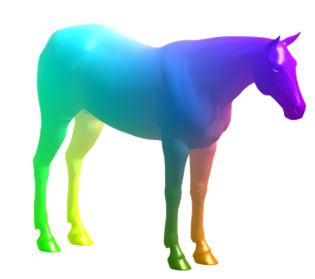
\includegraphics[scale=0.5]{figures/horse_base.png} & 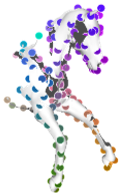
\includegraphics[scale=0.5]{figures/holes_horse_12_sparse.png} & 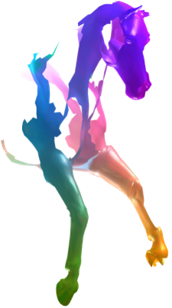
\includegraphics[scale=0.5]{figures/holes_horse_12.png} & 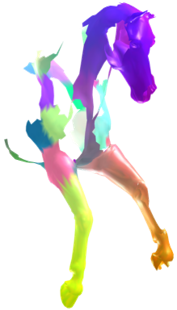
\includegraphics[scale=0.5]{figures/holes_horse_12_PFM.png}  & 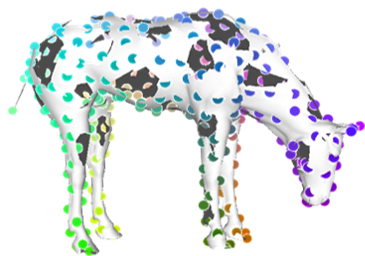
\includegraphics[scale=0.5]{figures/holes_horse_16_sparse.png} & 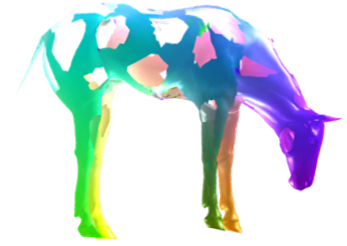
\includegraphics[scale=0.5]{figures/holes_horse_16.png} & 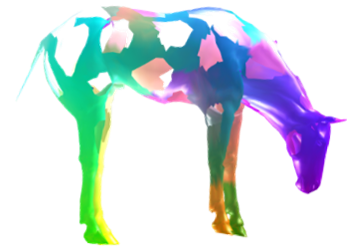
\includegraphics[scale=0.5]{figures/holes_horse_16_PFM.png}\\
	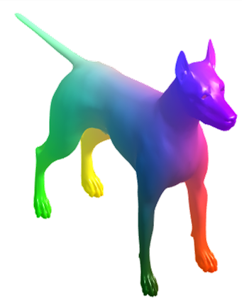
\includegraphics[scale=0.5]{figures/dog_base.png} &
	 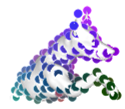
\includegraphics[scale=0.5]{figures/cuts_dog_8_sparse.png} & 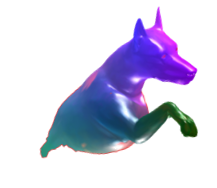
\includegraphics[scale=0.5]{figures/cuts_dog_8.png} & 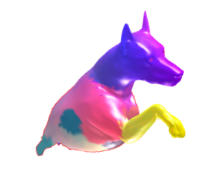
\includegraphics[scale=0.5]{figures/cuts_dog_8_PFM.png}  & 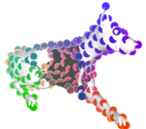
\includegraphics[scale=0.5]{figures/holes_dog_13_sparse.png} & 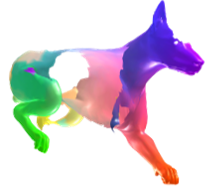
\includegraphics[scale=0.5]{figures/holes_dog_13.png} & 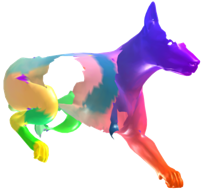
\includegraphics[scale=0.5]{figures/holes_dog_13_PFM.png}\\
	\end{tabular}
	\caption{{\bf Results on Shrec'16A.} 
	Our results outperform those of~\cite{rodola2017partial}, when run with the default parameters.
	\ayellet{(1) create little images (2) remove boundaries (3) change the model color in sparse correspondences (4) the models must be in the same size}\nadav{done}
	}
	\label{fig:Shrec16Qualitative}
\end{figure*}

Figure~\ref{fig:Shrec16Qualitative-error} further demonstrates it, by color-coding the errors.
The larger the error, the more reddish the color is.
\ayellet{add this figure}\nadav{done}
\begin{figure}[htb]

	\centering
	\setlength\tabcolsep{0.5pt}
	\begin{tabular}[width=0.8\textwidth]{cc|cc}
	 	Ours &  \cite{rodola2017partial}
		& Ours &  \cite{rodola2017partial}\\ \hline
		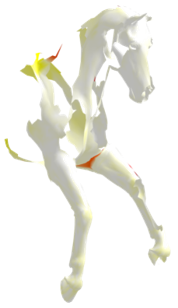
\includegraphics[scale=0.5]{figures/holes_horse_12_err.png} & 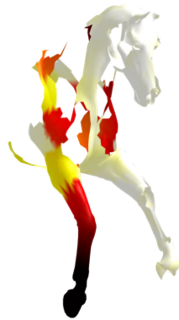
\includegraphics[scale=0.5]{figures/holes_horse_12_err_PFM.png} &  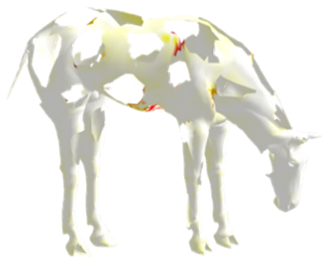
\includegraphics[scale=0.5]{figures/holes_horse_16_err.png} &  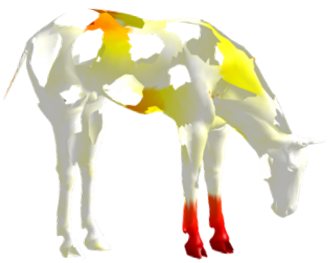
\includegraphics[scale=0.5]{figures/holes_horse_16_err_PFM.png}\\
		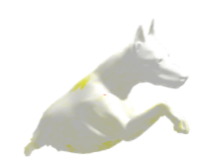
\includegraphics[scale=0.5]{figures/cuts_dog_8_err.png} & 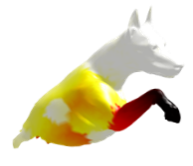
\includegraphics[scale=0.5]{figures/cuts_dog_8_err_PFM.png} &  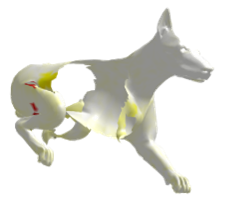
\includegraphics[scale=0.5]{figures/holes_dog_13_err.png} &  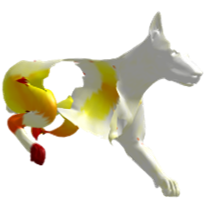
\includegraphics[scale=0.5]{figures/holes_dog_13_PFM_err.png}\\
	\end{tabular}
	\caption{{\bf Errors on SHREC'16A.} 
		\nadav{ Errors are coded from white(no error) to red. Our method outperforms that of~\cite{rodola2017partial}}
	}
	\label{fig:Shrec16Qualitative-error}
\end{figure}
Figure~\ref{fig:Shrec16TopImage} shows a couple of examples from the {\em SHREC'16B} dataset.
On the topological noise benchmark we can see bad matches are typically limited to the area of the topological noise, while PFM breaks completely on occasions.

\begin{figure}[htb]

	\centering
	\begin{tabular}{ccc}
	    base object & Ours & \cite{rodola2017partial}  
	    \\
	    	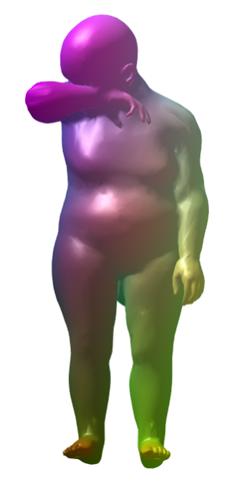
\includegraphics[scale=0.5]{figures/Top1Base.png} & 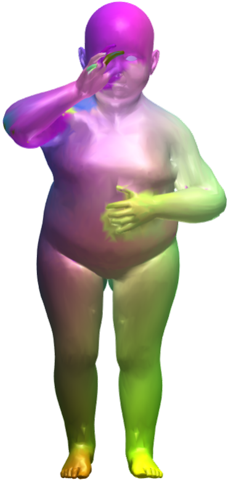
\includegraphics[scale=0.5]{figures/Top1DDIS.png} & 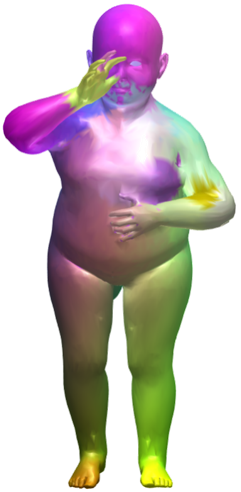
\includegraphics[scale=0.5]{figures/Top1PFM.png} \\ 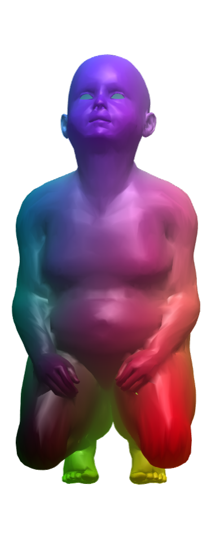
\includegraphics[scale=0.5]{figures/Top2Base.png} & 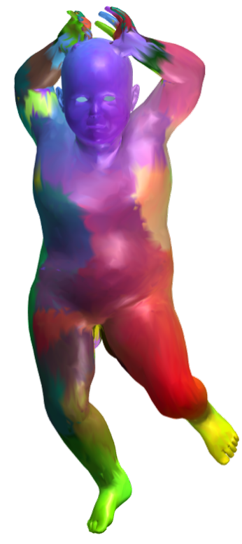
\includegraphics[scale=0.5]{figures/Top2DDIS.png} & 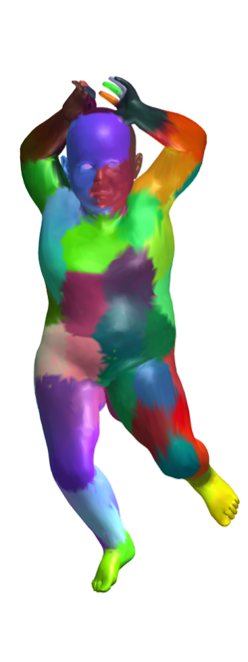
\includegraphics[scale=0.5]{figures/Top2PFM.png}
	\end{tabular}

	\caption{{\bf Results on Shrec'16B.} 
	Our results outperform those of~\cite{rodola2017partial}.}
	\label{fig:Shrec16TopImage}
\end{figure}

\nadav{TBA: Faust}

\paragraph{Quantitative results:}
Next, we provide quantitative evaluation of our method on the above datasets w.r.t previously reported results.
The common error metric used is the normalized geodesic distance~\cite{kim2011blended}.
Specifically, let the corresponding point of $(q \in \mathcal{N}$, as found by the algorithm, be $ p \in \mathcal{M})$ and let the ground truth corresponding point of $q$ be $p^* \in \mathcal{M})$. 
The error of for $q$ is the normalized geodesic distance between  $p$ and $p^*$ on $\mathcal{M}$:
\begin{equation}
\varepsilon(q)=\frac{GeoDist_{\mathcal{M}}(p,p^*)}{\sqrt{area(\mathcal{M})}}
\end{equation}

Figure~\ref{fig:Shrec16Cumulative} shows the cumulative curve, which indicates the percentage of errors falling below a varying geodesic threshold on {\em SHREC'16A}. 
% Symmetric solutions are accepted with no penalty.
The figure shows both sparse correspondences (dashed lines) and dense correspondences (solid lines), compared to other state-of-the-art algorithms~\cite{litany2017fully,rodola2017partial,sahillioglu2011coarse,rodola2013elastic,Rodola:2014:DNS:2679600.2679987,Torsello:2012:GAD:2354409.2354702,kovnatsky2013coupled},
\ayellet{add all references}\nadav{Done.}
as provided in the benchmark site. \ayellet{cite the site}\nadav{\hyperlink{url:shrec16A}{http://www.dais.unive.it/~shrec2016/}}
In both cases, our method considerably outperforms state-of-the-art algorithms, both on the subset of the dataset that contains models with holes and on the subset that contains partial models.
The obtained increase in performance in by $~10\%$ for the cuts subset and by $20\%$ for the holes subset.
% We compare them with the results reported in Fully Spectral Partial Matching(FSPM)\cite{litany2017fully}, which also compares results with partial functional maps(PFM)\cite{rodola2017partial}, random forests(RF), scale-invariant isometric matching(IM), game-theoretic matching(GT), elastic net matching(EN) and joint diagnolization. 

\begin{figure}[htb]
	\centering
		\setlength\tabcolsep{0.5pt}
	\begin{tabular}{ccc}
		& Cuts & Holes \\
		\rotatebox{90}{    \, \% Correspondences} &
		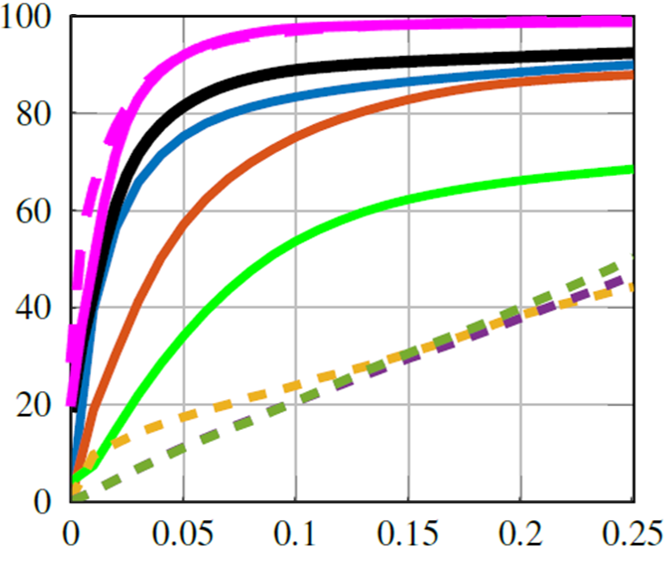
\includegraphics[scale=0.35]{figures/SHRECCutsCumulative16.png} & 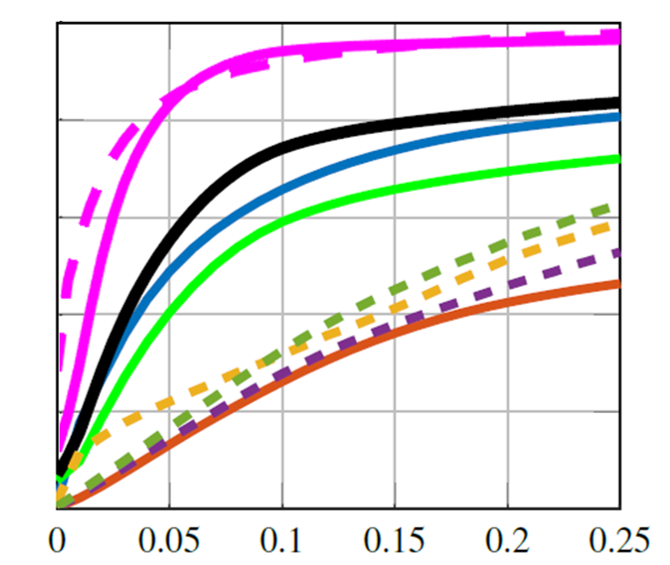
\includegraphics[scale=0.35]{figures/SHRECHolesCumulative16.png} \\
		& Geodesic Error & Geodesic Error\\
		\multicolumn{3}{c}{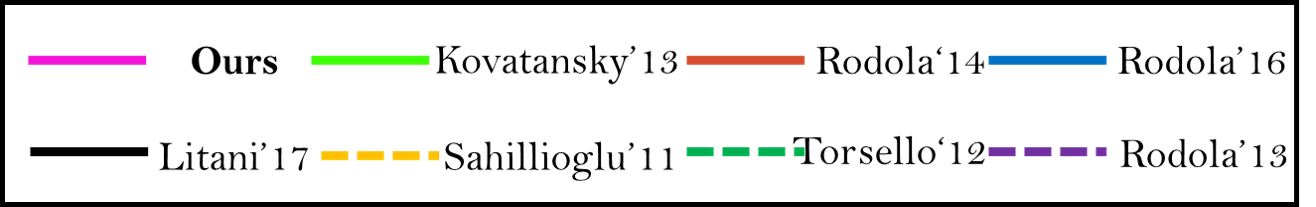
\includegraphics[width=0.5\textwidth]{figures/SHREC16Amethods.png}}
	\end{tabular}
	\caption{{\bf Cumulative geodesic error curves on Shrec16A.} 
	Our method (in magenta) outperforms other algorithms, both for the dense correspondence and for the sparse correspondence, on the two subsets of the dataset.
	\ayellet{1. three images, (2) [Author'19] or Ours}}
	\label{fig:Shrec16Cumulative}
\end{figure}

\ayellet{Add a paragraph describing Figure~\ref{fig:Shrec16Part}}
\nadav{Figure~\ref{fig:Shrec16Part} shows the mean geodesic error of the mapping from a partial model $\mathcal{N}$ to the full model $\mathcal{M}$ as a function of $area(\mathcal{N})/area(\mathcal{M})$, hereafter referred to as partiality. It can be seen that our method is weakly dependent on the partiality of the model.}
\begin{figure}[htb]

		\setlength\tabcolsep{0.5pt}
\begin{tabular}{ccc}
	& Cuts & Holes \\
	\rotatebox{90}{Mean Geodesic Error} &
	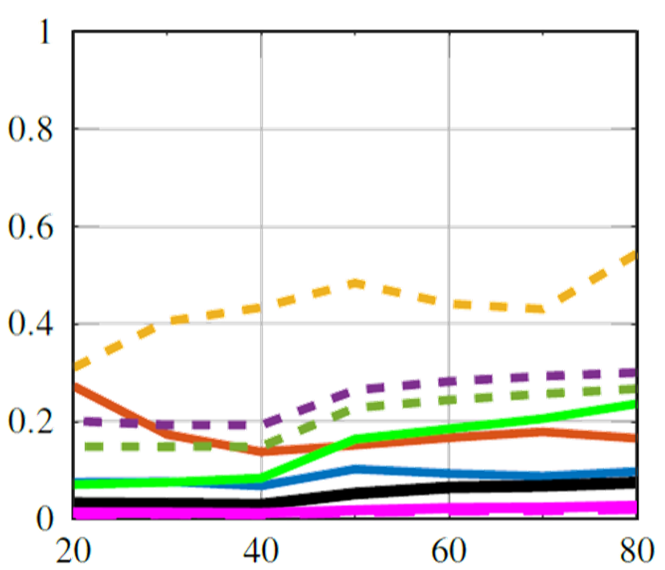
\includegraphics[scale=0.35]{figures/SHRECCutsPartiality16.png} & 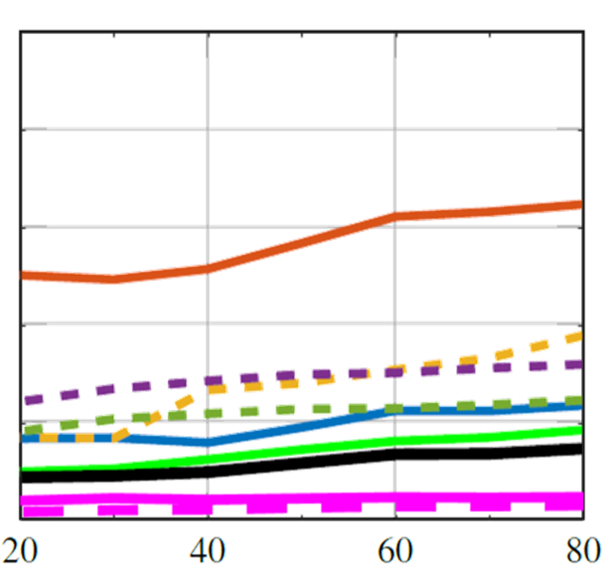
\includegraphics[scale=0.35]{figures/SHRECHolesPartiality16.png} \\
	& Partiality (\%) & Partiality (\%)\\
	\multicolumn{3}{c}{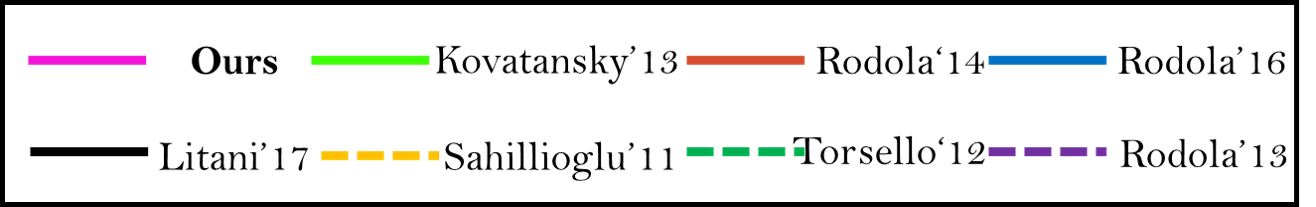
\includegraphics[width=0.5\textwidth]{figures/SHREC16Amethods.png}}
\end{tabular}
	\caption{Error as a function of model partiality.}
		\label{fig:Shrec16Part}
\end{figure}

Figure~\ref{fig:Shrec16Top} compares our results to results of state-of-the-art algorithms\cite{vestner2017efficient,litany2017fully,rodola2017partial,chen2015robust,sahilliouglu2012scale,Rodola:2014:DNS:2679600.2679987,cosmo2016shrec} for {\em SHREC'16B}.
Our method is competitive with that of~\cite{vestner2017efficient}, despite of the fact that our algorithm heavily depends on geodesic distances, and topological noise e.g., connecting the hand to the face) shortens these distances.
% We can see from the plot that we fall short of achieving state of the art results on this benchmark.
% The additional paths between points introduced by topological noise causes significant problems in matching, especially around the noisy areas, a fact that\cite{vestner2017efficient} manages to tackle partially by optimizing over different distance kernels along with descriptor similarity. 
% It might be worthwhile to find a way to incorporate these kernels into the 3D-DDIS framework.

\begin{figure}[htb]

	\centering
\setlength\tabcolsep{0.5pt}
\begin{tabular}{cc}
	\rotatebox{90}{    \, \% Correspondences} &
	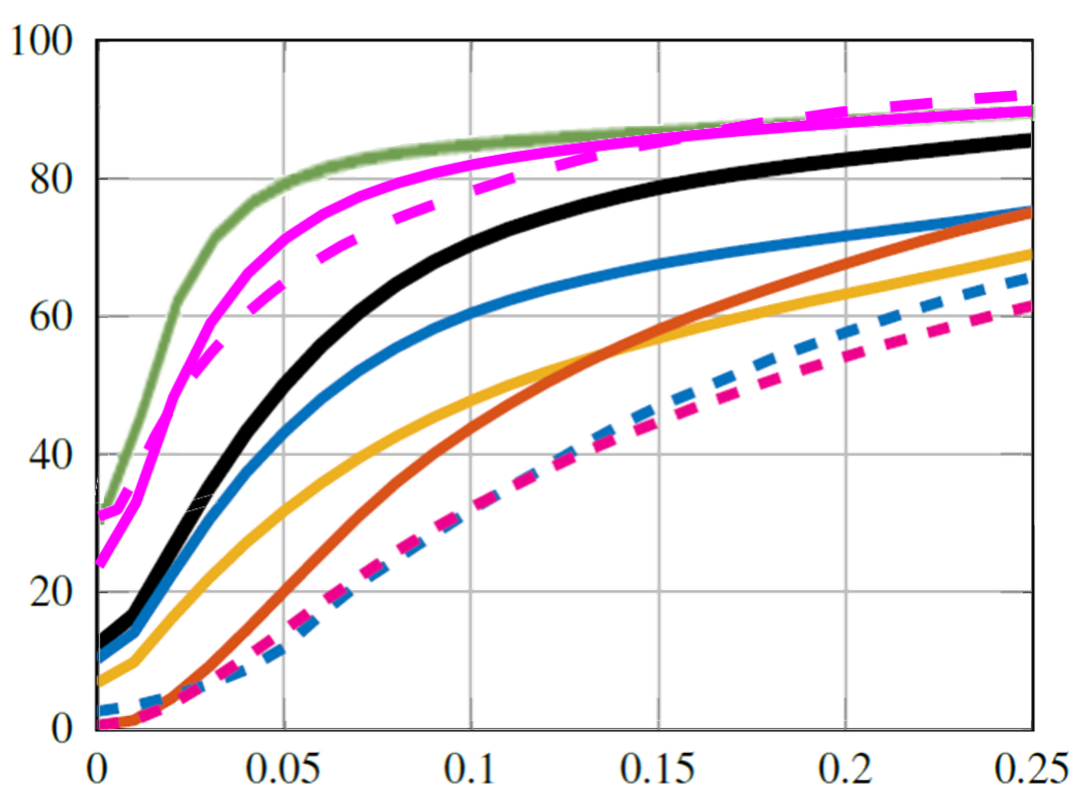
\includegraphics[scale=0.3]{figures/SHREC16BCummulative.png}\\
	& Geodesic Error \\
		\multicolumn{2}{c}{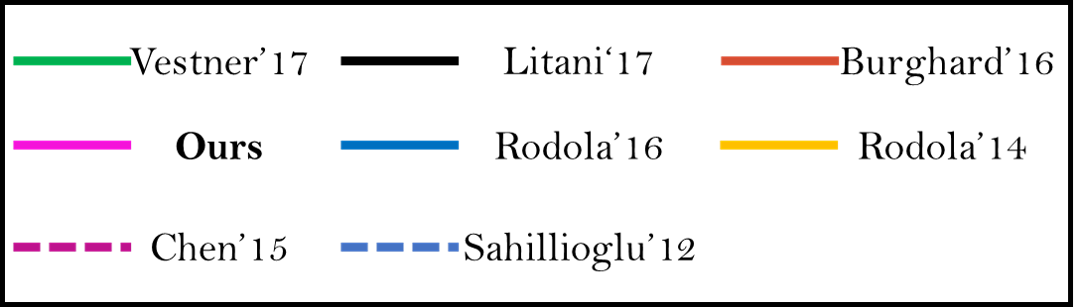
\includegraphics[width=0.35\textwidth]{figures/SHREC16Bmethods.png}}
\end{tabular}
	\caption{{\bf Cumulative error curve on SHREC'16B.} \ayellet{same changes to the figure}}
		\label{fig:Shrec16Top}
\end{figure}

\paragraph{Drawbacks:} xxx


\ayellet{fifth paragraph: drawbacks with examples}
\nadav{Our method exhibits a few drawbacks.
    First and foremost the algorithm has a high asymptotic runtime - $O(n^2logn) + O(|S|n^2)$(App.~\ref{app:Runtime}). 
	This limits the utilization of our method to relatively small shapes with less than ~15K vertices, which takes ~200s. 
	The algorithm also has six parameters which need to be tuned. 
	In addition,the algorithm has some typical failure cases that can be seen in Figure~\ref{fig:FailureCases}: 
	(1)Surface patches such as the dog's tail that are low in distinct shapes are hard to match. (2)Topological noise due to the intersection of different model parts changes the geodesic paths of the deformed model w.r.t to the base model.
(3) Extreme deformations can cause shape descriptors of the deformed model to be vastly different than those of the base model.}

\begin{figure*}[htb]
	\centering
\setlength\tabcolsep{0.5pt}
\begin{tabular}{cccccc}
	
	\multicolumn{2}{c}{a} & 	\multicolumn{2}{c}{b} & \multicolumn{2}{c}{c} \\ 
	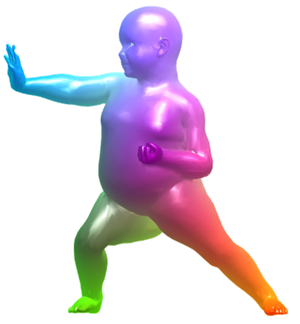
\includegraphics[scale=0.7]{figures/FailTopBase.png} &
	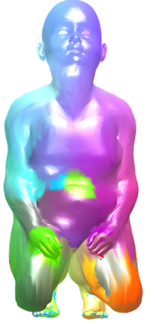
\includegraphics[scale=0.7]{figures/FailTopmatch.png} &
	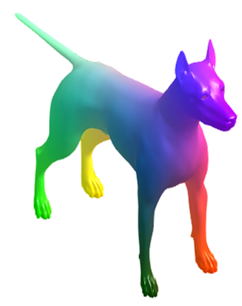
\includegraphics[scale=0.7]{figures/FailHolesbase.png} &
	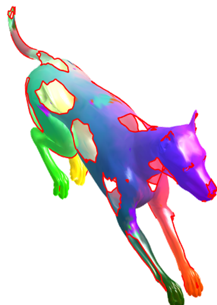
\includegraphics[scale=0.7]{figures/FailHolesmatch.png} &
	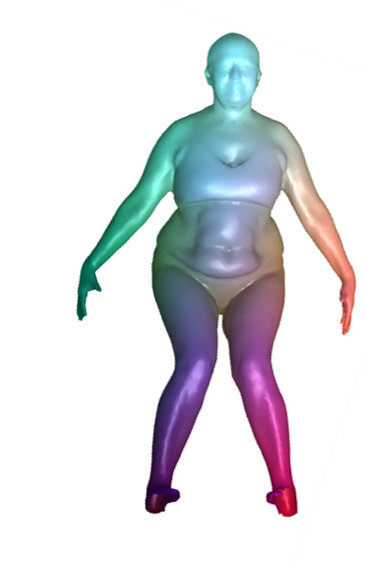
\includegraphics[scale=0.4]{figures/FailCutsbase.png} &
	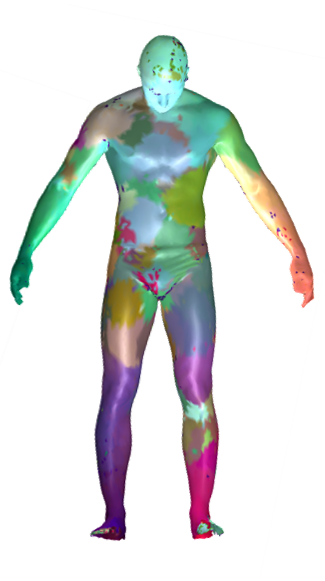
\includegraphics[scale=0.4]{figures/FailCutsMatch.png}
\end{tabular}
\caption{\nadav{Typical failure cases of our method.
		 (a) Strong topological noise affects geodesic distances, causing the right hand to be mapped to the leg.
		 (b) Narrow surfaces which contain a low number of points are harder to match.
	     (c)Extreme deformations make shape descriptors unreliable.}}
	\label{fig:FailureCases}
\end{figure*}

\paragraph{Implementation details:} xxx
\ayellet{sixth paragraph: implementation details, how do we move from sparse to dense}
\nadav{Our code which produces the sparse correspondences is implemented entirely in C++ . 
We have used the Fast Marching Method\cite{kimmel1996fast} to obtain geodesic distances.
FPFH shape descriptors are calculated using the Point Cloud library\cite{Rusu_ICRA2011_PCL}. 
The Nearest Neighbor field is computed with FLANN\cite{muja2009fast} with $\chi^2$ distance.
The entire code is parallelized using OpenMP. Since computing similarity for a given patch is totally independent from its calculation for other patches, the obtained speedup is nearly linear in the number of threads. 
}

\nadav{
To move from sparse to dense correspondence we employ the method of \cite{litany2017fully}. 
We had replaced the input dense descriptor field with localized smooth delta functions around our corresponding pairs.
We have found that satisfying results are already achieved after 1 iteration on SHREC16'A, and 2 on SHREC'16B. We have tuned the parameters of \cite{litany2017fully} on 15 models of cats from the SHREC16'A training set.}


\paragraph{Alternatives:} 
\ayellet{sixth paragraph: alternatives---comparison to Lihi's function}
\nadav{I have moved this to the end - it is difficult to write as we didn't introduce their formulation...}

\nadav{ We have used the training set provided with SHREC'16A to experiment with different variations and parameters of our method, which will be described hereafter.}

\nadav{\textit{Coherency based refinement} We evaluate the effect of our coherency based refinement on the SHREC16'A training set. A qualitative comparison is shown in Figure~\ref{fig:CoherencyQual}. The quantitative comparison in Figure~\ref{fig:CoherencyQuant}   shows an improvement of 1.5\% additional matches which fall below the 5\% threshold.}

\begin{figure}[htb]
	\centering
	\begin{tabular}{ccc}
		base object & Before & After  
		\\
		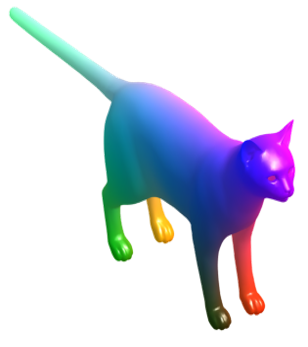
\includegraphics[scale=0.7]{figures/cat_base.png} & 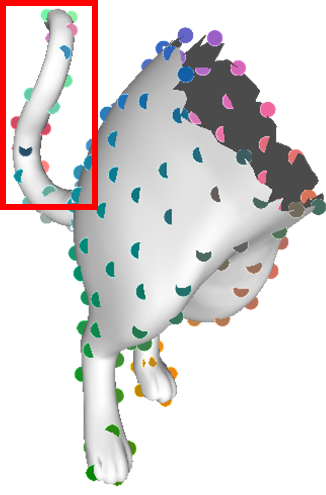
\includegraphics[scale=0.4]{figures/cat_7_non_greedy.png} & 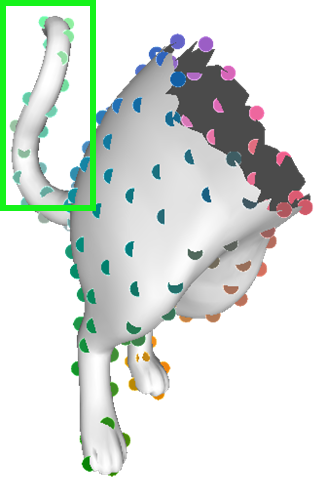
\includegraphics[scale=0.4]{figures/cat_7_greedy.png} \\ 
	\end{tabular}
	
	\caption{\nadav{{\bf Coherency based refinement.} 
		The outlier incoherent matches on the cat's tail got replaced by the coherent and correct ones.}}
	\label{fig:CoherencyQual}
\end{figure}

\begin{figure}[htb]
	\centering
	\setlength\tabcolsep{0.5pt}
	\begin{tabular}{cc}
		\rotatebox{90}{    \, \% Correspondences} &
		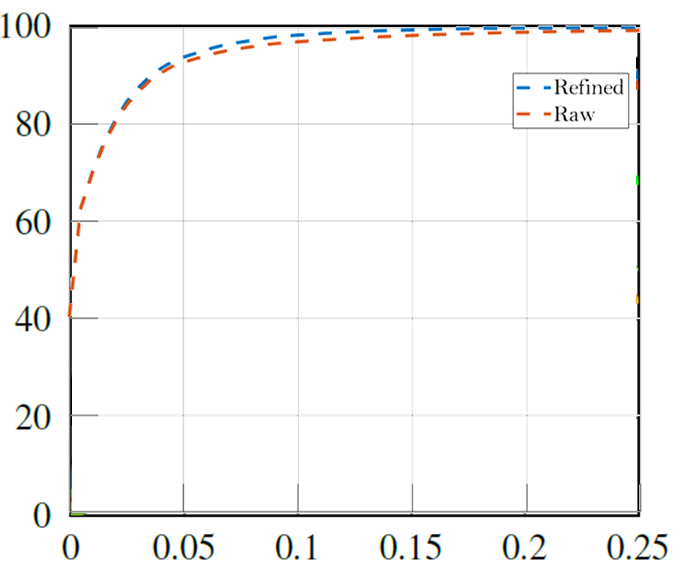
\includegraphics[scale=0.4]{figures/CoherencyRefinement.png}\\
		& Geodesic Error \\
	\end{tabular}
	\caption{\nadav{{\bf Coherency based refinement} quantitative comparison. A 1.5\% improvement is achieved}}
	\label{fig:CoherencyQuant}
\end{figure}


\paragraph{Robustness:} 
\ayellet{parameter tuning}
\nadav{
\textit{Surface patch radius} We have explored the behaviour of 3DDIS given different values of the surface patch radius $R_T$. 
The effects of different choices are illustrated in Figure~\ref{fig:DifferentRadii}.
It can be seen that in general, a smaller surface radius leads to results which are better locally, as evident from the higher percentage of matches below 0.1\% error. 
This, however, comes at the cost of some globally inconsistent matches, which cause this precentage to drop the farther along the curve we go.
The application of our multiscale framework results in an overall better result than any single scale alone.
\begin{figure*}[htb]

	\centering
	\setlength\tabcolsep{0.5pt}
	\begin{tabular}{cccc}
		& \textbf{(a)} & \textbf{(b)} & \textbf{(c)}\\
		\rotatebox{90}{    \, \% Correspondences} &
		\includegraphics[scale=0.5]{figures/PieceSizeLow.png} &  
		\includegraphics[scale=0.5]{figures/PieceSizeMedium.png}&
		\includegraphics[scale=0.5]{figures/PieceSizeHigh.png}
		\\
		& Geodesic Error &  Geodesic Error &  Geodesic Error\\
	\end{tabular}
	\caption{\nadav{{\bf A comparison of different piece radii}. (a) We can see that a radius of 20\%$\sqrt{area(\mathcal{M})}$ has the most correspondences with an error below the threshold 0.01\%.(b) shows a 40\% radius overtakes it near the 0.1\% mark.}} 
		\label{fig:DifferentRadii}
\end{figure*}
}

\nadav{
	\textit{Similarity formulation}	We have tested our 3DDIS formulation against the formulation of \cite{talmi2017template}. 
	The main difference between the two is as follows:
	The similarity metric of\cite{talmi2017template}, expects the NNF to be nearly bijective.
	Thus, it penalizes the similarity score of a point in $P$ being a nearest neighbor of multiple points in $Q$. 
	The comparison, illustrated in Figure~\ref{fig:OriginalDDIS} shows a significant improvement over the original formulation. stemming from a higher robustness to partiality. Figure~\ref{fig:OriginalDDIS}b implies that 3DDIS handles high model partiality better.}

\begin{figure}[htb]
	\centering
	\setlength\tabcolsep{0.5pt}
	\begin{tabular}{cccc}
		& \textbf{(a)} & & \textbf{(b)} \\
		\rotatebox{90}{    \, \% Correspondences} &
		\includegraphics[scale=0.7]{figures/DDISvs3DDISCumulative.png} & 
		\rotatebox{90}{Mean Geodesic Error} & 
		\includegraphics[scale=0.7]{figures/DDISv3DDISPartial.png}
		\\
		& Geodesic Error & & Partiality(\%)\\
	\end{tabular}
	\caption{\nadav{\bf A comparison between Our formulation and the original DDIS. (a) Shows a 5
	\% improvement in match quality. (b) shows our formulation can tackle cases of extreme partiality better.} \ayellet{same changes to the figure}\nadav{done}}
	\label{fig:OriginalDDIS}
\end{figure}

\paragraph{Applications:} xxx
\ayellet{seventh paragraph: uses in archaeology}
\nadav{We have also used 3DDIS to detect repeating patterns in archaeological artifact. 
Here we first found the geodesic center of the desired pattern in the scene, and extracted the geodesic disc around it.
Then we employed our DDIS pipeline between our part and the geodesic disc. TBA -figures}


{\small
\bibliographystyle{ieee}
\bibliography{egbib}}


\begin{appendices}
\chapter{Some Appendix}
The contents...
\end{appendices}
\paragraph{Appendix A: Runtime and complexity}
\label{app:Runtime}
\nadav{
	We calculate asymptotic runtime complexity using the following valid assumptions:
	(a)$|S|<<|\mathcal{M}|$ - this is satisfied since we only compute sparse correspondences typically <300 for a full model. 
	(b) $|\mathcal{N}|\approx |\mathcal{M}|=n$. 
	The complexity of different algorithm stages is thus:
}
\begin{enumerate}
	
	\item \nadav{\textit{FPFH Calculation} Calculation of FPFH takes $O(n \cdot k)$ where $k$ is the number of neighbors for each point in a defined spherical neighborhood of a radius $R_F$. In our case $R_F=0.03\sqrt{area(\mathcal{M})}$ which implies $k << n$ .
	}
	
	\item \nadav{\textit{NN search} Approximate nearest neighbor are calculated by building a kd-tree for $\mathcal{N}$ which takes $O(dnlogn)$, where $d$ is the feature dimension,
		In the case of FPFH, $d=33$ and is thus treated as a constant. 
		We perform a NN search for each vertex of $\mathcal{M}$, each taking $O(logn)$ operations. 
		Thus the overall complexity of this stage is $O(nlogn)$.}
	
	\item \nadav{\textit{Geodesics} Calculating fast marching geodesics distances from a single point to all other points on a mesh has a runtime complexity of $O(nlogn)$.
		Since we repeat this process for each point on both meshes the total complexity of this stage becomes $O(n^2logn)$}
	
	\item \nadav{\textit{Similarity map calculation} Calculation of similarity between a pair of patches $P,Q$, requires a single pass over all the points in both. 
		Thus, requires $O(|P|+|Q|)\approx O(n)$ operations. 
		We compute  similarity scores for all possible patches in $\mathcal{M}$ to all sample patches in $S$. 
		Overall we make $O(|S|n)$ similarity calculations. 
		Thus the runtime complexity of this stage has an upper bound of $O(|S|n^2)$ operations.}
	
	\item \nadav{\textit{Correspondence Refinement} 
		Detecting outliers is done in $O(|S|^2)$ - we sum the geodesic distance differences of each sample point to all other points on its respective model. 
		We set the numbers of alternative 3DDIS maximas to 100 for each point. This can be done in a linear time in $|S|$ for each sample, thus the maxima detection also requires $O(|S|^2)$ operations.
		Overall the stage has a runtime complexity of $O(|S|^2)$}.
	
\end{enumerate}
\nadav{In total, the algorithm has an effective runtime complexity of $O(|S|n^2) + O(n^2logn)$.
	As previously mentioned, this limits us to running on models of ~15,000k vertices. 
	Mesh simplification algorithms can be applied for downsampling if running on larger models is required.}


\end{document}